\chapter{Quantum phase estimation}\label{chap:qpe}

The setup of the phase estimation problem is as follows. 
Let $U$ be a unitary, and $\ket{\psi}$ is an eigenvector, i.e.,
\begin{equation}
U\ket{\psi}=e^{\I 2\pi \varphi} \ket{\psi}, \quad \varphi\in[0,1).
\label{eqn:qpe_objective}
\end{equation}
The goal is to find $\varphi$ up to certain precision.
This is a quantum primitive with numerous applications: prime factorization (Shor's algorithm), linear system (HHL), eigenvalue problem, amplitude estimation, quantum counting, quantum walk, etc.

Using a classical computer, we can estimate $\varphi$ using $U\ket{\psi}\oslash\ket{\psi}$, where $\oslash$ stands for the element-wise division operation.
Specifically, if $\ket{\psi}$ is indeed an eigenvector and $\braket{j|\psi}\ne 0$ for any $j$ in the computational basis, then we can extract the phase from
\begin{equation}
\braket{j|U|\psi}/\braket{j|\psi}=e^{\I 2\pi \varphi}.
\end{equation}
Unfortunately, such a element-wise division operation cannot be efficiently implemented on quantum computers, and alternative methods are needed.

Quantum phase estimation has numerous variants, and still receives intensive research attention till today. This chapter only introduces some of the simplest variants.


\section{Hadamard test}

We first introduce the Hadamard test, which is a useful tool for computing the expectation value of an unitary operator with respect to a state, i.e., $\braket{\psi|U|\psi}$.
Since $U$ is generally not Hermitian, this does not correspond to the measurement of a physical observable.
Instead the real and imaginary part of the expectation value need to be measured separately.

The (real) Hadamard test is the quantum circuit in \cref{fig:hadamard_real} for estimating the real part of $\braket{\psi|U|\psi}$.
\begin{figure}[H]
\begin{displaymath}
\begin{quantikz}
\lstick{$\ket{0}$} & \gate{H} & \ctrl{1}  & \gate{H} &\meter{}\\
\lstick{$\ket{\psi}$} & \qwb           & \gate{U}  & \qw & \qw
\end{quantikz}
\end{displaymath}
\caption{Hadamard test for $\Re \braket{\psi|U|\psi}$.}
\label{fig:hadamard_real}
\end{figure}

To verify this, we find that the circuit transforms $\ket{0}\ket{\psi}$ as
\begin{displaymath}
\begin{split}
\ket{0}\ket{\psi} \xrightarrow{\mathrm{H}\otimes I} & \frac{1}{\sqrt{2}}(\ket{0}+\ket{1})\ket{\psi}\\
\xrightarrow{c\text{-}U} & \frac{1}{\sqrt{2}}(\ket{0}\ket{\psi}+\ket{1}U\ket{\psi})\\
\xrightarrow{\mathrm{H}\otimes I} & \frac{1}{2}\ket{0}(\ket{\psi}+U\ket{\psi})+
\frac{1}{2}\ket{1}(\ket{\psi}-U\ket{\psi}).
\end{split}
\end{displaymath}
The probability of measuring the qubit $0$ to be in state $\ket{0}$ is 
\begin{equation}
p(0)=\frac{1}{2}(1+\Re \braket{\psi|U|\psi}).
\end{equation}
This is well defined since $-1\le \Re \braket{\psi|U|\psi}\le 1$.

To obtain the imaginary part, we can use the circuit in \cref{fig:hadamard_imag} called the (imaginary) Hadamard test, where
\begin{equation} 
S=\begin{pmatrix}
1 & 0\\
0 & \I
\end{pmatrix}
\end{equation}
is called the phase gate.

\begin{figure}[H]
\begin{displaymath}
\begin{quantikz}
\lstick{$\ket{0}$} & \gate{H} & \gate{S^{\dag}} &\ctrl{1}  & \gate{H} &\meter{}\\
\lstick{$\ket{\psi}$} & \qwb           & \qw & \gate{U}  & \qw & \qw
\end{quantikz}
\end{displaymath}
\caption{Hadamard test for $\Im \braket{\psi|U|\psi}$.}
\label{fig:hadamard_imag}
\end{figure}

Similar calculation shows the circuit transforms $\ket{0}\ket{\psi}$ to the state
\begin{equation}
\frac{1}{2}\ket{0}(\ket{\psi}-\I U\ket{\psi})+
\frac{1}{2}\ket{1}(\ket{\psi}+\I U\ket{\psi}).
\end{equation}
Therefore the probability of measuring the qubit $0$ to be in state $\ket{0}$ is 
\begin{equation}
p(0)=\frac{1}{2}(1+\Im \braket{\psi|U|\psi}).
\end{equation}
Combining the results from the two circuits, we obtain the estimate to $\braket{\psi|U|\psi}$.

 
\begin{exam}[Overlap estimate using swap test]
An application of the Hadamard test is called the swap test, which is used to estimate the overlap of two quantum states $\abs{\braket{\varphi|\psi}}$.
The quantum circuit for the swap test is
\begin{figure}[H]
\begin{displaymath}
\begin{quantikz}
\lstick{$\ket{0}$} & \gate{H} & \ctrl{2}  & \gate{H} &\meter{}\\
\lstick{$\ket{\varphi}$} & \qwb           & \swap{1}  & \qw & \qw\\
\lstick{$\ket{\psi}$} & \qwb           & \targX{}  & \qw & \qw
\end{quantikz}
\end{displaymath}
\caption{Circuit for the SWAP test.}
\label{fig:circuit_swap}
\end{figure}
Note that this is exactly the Hadamard test with $U$ being the $n$-qubit swap gate.
Direct calculation shows that the probability of measuring the qubit $0$ to be in state $\ket{0}$ is 
\begin{equation}
p(0)=\frac{1}{2}(1+\Re \braket{\varphi,\psi|\psi,\varphi})=\frac12(1+\abs{\braket{\varphi|\psi}}^2).
\end{equation}
\end{exam}

\begin{exam}[Overlap estimate with relative phase information]
\label{exam:swap_test}
In the swap test, the quantum states $\ket{\varphi},\ket{\psi}$ can be black-box states, and in such a scenario obtaining an estimate to $\abs{\braket{\varphi|\psi}}$ is the best one can do.
In order to retrieve the relative phase information and to obtain $\braket{\varphi|\psi}$, we need to have access to the unitary circuit preparing  $\ket{\varphi},\ket{\psi}$, i.e.,
\begin{equation}
U_{\varphi}\ket{0^n}=\ket{\varphi}, \quad U_{\psi}\ket{0^n}=\ket{\psi}.
\end{equation}
Then we have $\braket{\varphi|\psi}=\braket{0^n|U_{\varphi}^{\dag}U_{\psi}|0^n}$.
\end{exam}

\begin{exam}[Single qubit phase estimation]\label{exam:singlequbit_pe}
The Hadamard test can also be used to derive the simplest version of the phase estimate based on success probabilities.
Apply the Hadamard test in \cref{fig:hadamard_real} with $U,\psi$ satisfying \cref{eqn:qpe_objective}. Then the probability of measuring the qubit $0$ to be in state $\ket{1}$ is 
\begin{equation}
p(1)=\frac{1}{2}(1-\Re \braket{\psi|U|\psi})=\frac{1}{2}(1-\cos (2\pi\varphi)).
\end{equation}
Therefore
\begin{equation}
\varphi=\pm\frac{\arccos(1-2p(1))}{2\pi} \pmod{1}.
\end{equation}
In order to quantify the efficiency of the procedure, recall from \cref{exam:prob_onequbit} that if $p(1)$ is far away from  $0$ or $1$, i.e., $(2\varphi \mod 1)$ is far away from $0$, in order to approximate $p(1)$ (and hence $\varphi$) to additive precision $\epsilon$, the number of samples needed is $\Or(1/\epsilon^2)$.

Now assume $\varphi$ is very close to $0$ and we would like to estimate $\varphi$ to additive precision $\epsilon$. Note that
\begin{equation}
p(1)\approx (2\pi\varphi)^2 = \Or(\epsilon^2).
\end{equation}
Then $p(1)$ needs to be estimated to precision $\Or(\epsilon^2)$, and again the number of samples needed is $\Or(1/\epsilon^2)$. The case when $\varphi$ is close to $1/2$ or $1$ is similar.

Note that the circuit in \cref{fig:hadamard_real} cannot distinguish the sign of $\varphi$ (or  whether $\varphi\ge 1/2$ when restricted to the interval $[0,1)$).
To this end we need \cref{fig:hadamard_imag}, but replace $\mathrm{S}^{\dag}$ by $\mathrm{S}$, so that the success probability of measuring $1$ in the computational basis is
\begin{equation} 
p(1)=\frac{1}{2}(1+\sin(2\pi\varphi)).
\end{equation}
This gives
\begin{equation}
 \varphi
\begin{cases}
\in[0,1/2), & p(1)\ge \frac12,\\
\in(1/2,1),    & p(1)< \frac12.
\end{cases}
\end{equation}
Unlike the previous estimate, in order to correctly estimate the sign, we only require $\Or(1)$ accuracy, and run \cref{fig:hadamard_imag} for a constant number of times (unless $\varphi$ is very close to $0$ or $\pi$).
\end{exam}

\begin{exam}[Qiskit example for phase estimation using the Hadamard test]
\label{exam:qpe_hadamard}
Here is a qiskit example of the simple phase estimation for

\[
R|1\rangle = 
\begin{pmatrix}
1 & 0\\
0 & e^{i2\pi\varphi}\\ 
\end{pmatrix}
\begin{pmatrix}
0\\
1\\ 
\end{pmatrix}
= e^{\I2\pi\varphi}|1\rangle,
\]
with $\varphi=0.5+\frac{1}{2^d}\equiv 0.{10\cdots 01}$ (d bits in total). In this example, $d=4$ and the exact value is $\varphi=0.5625$. 
\begin{center}
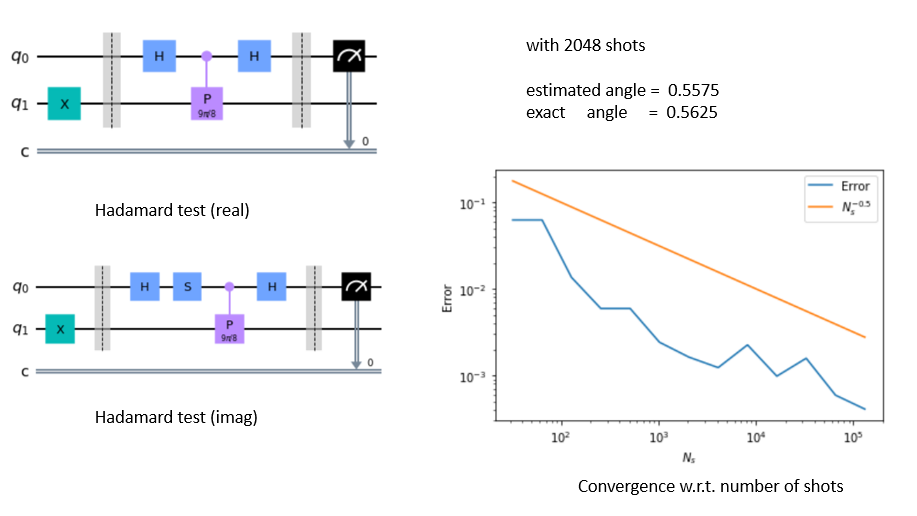
\includegraphics[width=0.8\textwidth]{phase_result_hadamard}
\end{center}

\end{exam}

\section{Quantum phase estimation (Kitaev's method)*}

In \cref{exam:singlequbit_pe}, the number of measurements needed to estimate $\varphi$ to precision $\epsilon$ is $\Or(1/\epsilon^2)$.
A quadratic improvement in precision (i.e., $\Or(1/\epsilon)$) can be achieved by means of the quantum phase estimation. One such procedure is called Kitaev's method~\cite[Section 13.5]{KitaevShenVyalyi2002}.

In the fixed point representation in \cref{sec:fixedpoint}, for simplicity we assume that the eigenvalue can be exactly represented using $d$ bits, i.e.,
\begin{equation}
\varphi=(.\varphi_{d-1}\cdots\varphi_0).
\end{equation}
In the simplest scenario, we assume $d=1$, and $\varphi=.\varphi_0,\varphi_0\in\{0,1\}$.
Then $e^{\I2 \pi  \varphi}=e^{\I \pi \varphi_0}$.

Performing the real Hadamard test in \cref{exam:singlequbit_pe}, we have $p(1)=0$ if $\varphi_0=0$, and $p(1)=1$ if $\varphi_0=1$. 
In either case, the result is \emph{deterministic}, and one measurement is sufficient to determine the value of $\varphi_0$.

Next, consider $\varphi=.\underbrace{0\cdots 0\varphi_0}_{d \mbox{ bits}}$. To determine the value of $\varphi_0$, we need to reach precision $\epsilon<2^{-d}$. The method in \cref{exam:singlequbit_pe} requires $\Or(1/\epsilon^2)=\Or(2^{2d})$ repeated measurements, or number of queries to $U$.
The observation from Kitaev's method is that if we can have access to $U^j$ for a suitable power $j$, then the number of queries to $U$ can be reduced.
More specifically, if we can query $U^{2^{d-1}}$, then the circuit in \cref{fig:kitaev_example} with $j=d-1$ gives
\begin{equation} 
p(1)=\frac{1}{2}(1-\cos (2\pi.\varphi_0))=
\begin{cases}
0, &\varphi_0=0,\\
1, &\varphi_0=1.
\end{cases}
\end{equation}
The result is again deterministic. 
Therefore the total number of queries to $U$ becomes $\Or(2^{-d})=\Or(\epsilon^{-1})$.

\begin{figure}[H]
\begin{displaymath}
\begin{quantikz}
\lstick{$\ket{0}$} & \gate{H} & \ctrl{1}  & \gate{H} &\meter{}\\
\lstick{$\ket{\psi}$} & \qwb           & \gate{U^{2^{j}}}  & \qw & \qw
\end{quantikz}
\end{displaymath}
\caption{Circuit used in Kitaev's method. Another one with a phase gate to determine the sign of $2^j \varphi$ may also be used.}
\label{fig:kitaev_example}
\end{figure}

This is the basic idea behind Kitaev's method: use a more complex quantum circuit (and in particular, with a larger circuit depth) to reduce the \emph{total} number of queries. 
As a general strategy, instead of estimating $\varphi$ from a single number, we assume access to $U^{2^j}$, and estimate $\varphi$ bit-by-bit.
In particular, changing $U\to U^{2^j}$ in the Hadamard test allows us to estimate
\begin{equation}
2^j \varphi=\varphi_{d-1}\cdots \varphi_{d-j}.\varphi_{d-j-1}\cdots\varphi_0= .\varphi_{d-j-1}\cdots\varphi_0 \pmod{1}
\end{equation}
One immediate difficulty of the bit-by-bit estimation is that we need to tell $0.0111\ldots$ apart from $0.1000\ldots$, and the two numbers can be arbitrarily close to each other (though the two numbers can also differ at some number of digits), and some careful work is needed. 
We will first describe the algorithm, and then analyze its performance.
The algorithm works for any $\varphi$, and then the goal is to estimate its $d$ bits.
For simplicity of the analysis, we assume $\varphi$ is exactly represented by $d$ bits. We will use extensively the distance
\begin{equation}\label{eqn:modone_dist}
\abs{x}_1\equiv\abs{x}_{\bmod 1}:=\min\{(x \bmod 1),1-(x \bmod 1)\},
\end{equation}
which is the distance on the unit circle.


First, by applying the circuit in \cref{fig:kitaev_example} (and the corresponding circuit to determine the sign) with $j=0,1,\ldots,d-3$, for each $j$ we can estimate $p(0)$, so that the error in $2^j\varphi$ is less than $1/16$ for all $j$ (this can happen with a sufficiently high success probability. For simplicity, let us assume that this happens with certainty).
The measured result is denoted by $\alpha_j$. 
This means that any perturbation must be due to the $5$th digit in the binary representation. For example, if $2^j\varphi=0.11100$, then $\alpha_j=0.11011$ is an acceptable result with an error $0.00001=1/32$, but $\alpha_j=0.11110$ is not acceptable since the error is $0.0001=1/16$. We then \textit{round} $\alpha_j$ $\pmod 1$ by its closest $3$-bit estimate denoted by $\beta_j$, i.e., $\beta_j$ is taken from the set $\set{0.000,0.001,0.010,0.011,0.100,0.101,0.110,0.111}$.  Consider the example of $2^j\varphi=0.11110$, if $\alpha_j=0.11101$, then $\beta_j=0.111$. But if $\alpha_j=0.11111$, then $\beta_j=0.000$. 
Another example is $2^j\varphi=0.11101$, if $\alpha_j=0.11110$, then both $\beta_j=0.111$ (rounded down) and $\beta_j=0.000$ (rounded up) are acceptable. We can pick one of them at random. We will show later that the uncertainty in $\alpha_j,\beta_j$ is not detrimental to the success of the algorithm.

Second, we perform some post-processing. Start from $j=d-3$, we can estimate $.\varphi_2\varphi_1\varphi_0$ to accuracy $1/16$, which recovers these three bits exactly.  The values of these three bits will be taken from $\beta_{d-3}$ directly. Then we proceed with the iteration: for $j=d-4,\ldots,0$, we assign
\begin{equation}\label{eqn:kitaev_decidephi}
\varphi_{d-j-1}=\begin{cases}
0,& \abs{.0\varphi_{d-j-2}\varphi_{d-j-3}-\beta_j}_{\bmod 1}<1/4,\\
1,& \abs{.1\varphi_{d-j-2}\varphi_{d-j-3}-\beta_j}_{\bmod 1}<1/4.
\end{cases}
\end{equation}
Here $\abs{\cdot}_{\bmod 1}$ is the periodic distance on $[0,1)$ and its value is always $\le 1/2$. 
Since the two possibilities are separated by $1/2$, for each $j$, there will be at most one case that is satisfied. We will also show that in all circumstances, there is always one case that is satisfied, regardless of the ambiguity of the choice of $\beta_j$ above.

After running the algorithm above, we recover $\varphi=.\varphi_{d-1}\cdots \varphi_0$ exactly. The total cost of Kitaev's method measured by the number of queries to $U$ is $\Or\left(\sum_{j=0}^{d-3} 2^{j}\right)=\Or(\epsilon^{-1})$.

If $\varphi$ is exactly represented by $d$ bits, we will obtain an estimate
\begin{equation}\label{eqn:phi_kitaev_estimate}
\abs{.\varphi_{d-1}\cdots \varphi_0-\varphi}_{\bmod 1}<2^{-d}=\epsilon.
\end{equation} 


% 
% First at $k=0$, we run the (real and imaginary) Hadamard  test with $U$ to constant precision, and obtain the estimate for the two leading digits $\varphi_{d-1},\varphi_{d-2}$.
% 
% Next, for $k=1,\ldots,d-2$, we run the (real) Hadamard test with $U\to U^{2^k}$ to constant precision. This allows us to estimate the phase of the next \emph{three} bits:
% \begin{equation}
% .\underbracket{\varphi_{d-k-1}\varphi_{d-k-2}\varphi_{d-k-3}}\cdots\varphi_0 \pmod{1}.
% \end{equation}
% Note that the real Hadamard test cannot distinguish the first bit (which is a sign). So the value of $\varphi_{d-k-1}$ has already been determined from the previous stage. Then we also need the value of $\varphi_{d-k-3}$ in order to determine $\varphi_{d-k-2}$ in the presence of rounding. This is why each step requires us to focus on three bits at a time.
% 
% Repeating this procedure, we can determine all values in the fixed precision representation $\varphi=.\varphi_{d-1}\cdots\varphi_0$. 


\begin{exam}
Consider $\varphi=0.\varphi_4\varphi_3\varphi_2\varphi_1\varphi_0=0.11111$ and $d=5$. Running Kitaev's algorithm with $j=0,1,2$ gives the following possible choices of $\beta_j$:
\[
\begin{array}{c|c|c}\hline
j & 2^j \varphi & \mbox{possible }\beta_j \\\hline
0 & 0.11111 & \set{0.111,0.000} \\\hline
1 & 0.1111 & \set{0.111,0.000} \\\hline
2 & 0.111 & \set{0.111} \\\hline
\end{array}
\]
Start with $j=2$. We have only one choice of $\beta_j$, and can recover $0.\varphi_2\varphi_1\varphi_0=0.111$. Then for $j=1$,  we need to use \cref{eqn:kitaev_decidephi} to decide $\varphi_3$. If we choose $\beta_j=0.111$, we have $\varphi_3=1$. But if we choose $\beta_j=0.000$, we still need to choose $\varphi_3=1$, since 
$\abs{.011-0.000}_{\bmod 1}=0.100=1/2>1/4$, and $\abs{.111-0.000}_{\bmod 1}=0.001=1/8<1/4$. 
Similar analysis shows that for $j=0$ we have $\varphi_4=1$. This recovers $\varphi$ exactly.
\end{exam}

\begin{exam}[A variant of Kitaev's algorithm that does not work]
Let us modify Kitaev's algorithm as follows: for each $2^j \varphi$ is determined to precision $1/8$, and round the result to $\beta_j\in\set{0.00,0.01,0.10,0.11}$. Start from $j=d-2$, we estimate $.\varphi_1\varphi_0$ exactly. Then for $j=d-3,\ldots,0$, we assign
\begin{equation}\label{eqn:kitaev_decidephi_2}
\varphi_{d-j-1}=\begin{cases}
0,& \abs{.0\varphi_{d-j-2}-\beta_j}_{\bmod 1}<1/2,\\
1,& \abs{.1\varphi_{d-j-2}-\beta_j}_{\bmod 1}<1/2.
\end{cases}
\end{equation}
Now that the inequality $<1/2$ above can be equivalently written as $\le 1/4$.
  
Let us run the algorithm above for $\varphi=0.\varphi_4\varphi_3\varphi_2\varphi_1\varphi_0=0.1111$ and $d=4$. This gives:
\[
\begin{array}{c|c|c}\hline
j & 2^j \varphi & \mbox{possible }\beta_j \\\hline
0 & 0.1111 & \set{0.11,0.00} \\\hline
1 & 0.111 & \set{0.11,0.00} \\\hline
2 & 0.11 & \set{0.11} \\\hline
\end{array}
\]
Start with $j=2$. We have only one choice of $\beta_j$, and can recover $0.\varphi_1\varphi_0=0.11$. Then for $j=1$, if we choose $\beta_j=0.11$, we have $\varphi_2=1$. But if we choose $\beta_j=0.00$, then 
$\abs{.01-0.00}_{\bmod 1}=0.0.01=1/4$, and $\abs{.11-0.000}_{\bmod 1}=0.01=1/4$. So the algorithm cannot distinguish the two possibilities and fails.
\end{exam}

Let us now  inductively show why Kitaev's algorithm works. Again assume $\varphi$ is exactly represented by $d$ bits. For $j=d-3$, we know that $\varphi_2\varphi_1\varphi_0$ can be recovered exactly. Then assume $\varphi_{d-j-2}\cdots\varphi_0$ have all been exactly computed, at step $j$ we would like to determine the value of $\varphi_{d-j-1}$. From
\begin{equation}
\abs{\alpha_j-2^j\varphi}_{\bmod 1}<1/16, \quad \abs{\alpha_j-\beta_j}_{\bmod 1}\le 1/16,
\end{equation}
we know
\begin{equation}
\abs{2^j\varphi-\beta_j}_{\bmod 1}< 1/8.
\end{equation}
Then 
\begin{equation}
\begin{split}
 &\abs{.\varphi_{d-j-1}\varphi_{d-j-2}\varphi_{d-j-3}-\beta_j}_{\bmod 1}\\
\le &
\abs{.\varphi_{d-j-1}\varphi_{d-j-2}\varphi_{d-j-3}-2^j\varphi}_{\bmod 1}
+
\abs{2^j\varphi-\beta_j}_{\bmod 1}\\
\le & 1/16+1/8<1/4.
\end{split}
\end{equation}
The wrong choice of $\varphi_{d-j-1}$ denoted by  $\wt{\varphi}_{d-j-1}$ then satisfies
\begin{equation}
\begin{split}
 &\abs{.\wt{\varphi}_{d-j-1}\varphi_{d-j-2}\varphi_{d-j-3}-\beta_j}_{\bmod 1}\\
\ge &
\abs{.\wt{\varphi}_{d-j-1}\varphi_{d-j-2}\varphi_{d-j-3}-.\varphi_{d-j-1}\varphi_{d-j-2}\varphi_{d-j-3}}_{\bmod 1}-
\abs{.\varphi_{d-j-1}\varphi_{d-j-2}\varphi_{d-j-3}-\beta_j}_{\bmod 1}\\
> & 1/2-1/4=1/4.
\end{split}
\end{equation}
This proves the validity of \cref{eqn:kitaev_decidephi}, and hence that of Kitaev's algorithm.


% \begin{exam}[Qiskit example for phase estimation using Kitaev's algorithm]
% The setup is the same as in \cref{exam:qpe_hadamard}.
% \begin{center}
% \includegraphics[width=1.0\textwidth]{phase_result_kitaev}
% \end{center}
% \end{exam}



\section{Quantum Fourier transform}

Fourier transform is used ubiquitously in scientific computing, and fast Fourier transform (FFT) is the backbone for many fast algorithms in classical computation.
Similarly, the quantum Fourier transform is also an important component in many quantum algorithms, such as phase estimation, Shor's algorithm, and inspires other fast algorithms such as fast Fermionic Fourier transform (FFFT) etc.

For any $j$ in the computational basis, the (discrete) forward Fourier transform is defined as
\begin{equation}
U_{\mathrm{FT}}\ket{j}=\frac{1}{\sqrt{N}}\sum_{k\in [N]} e^{\I 2\pi\frac{kj}{N}} \ket{k}.
\end{equation}
In particular
\begin{equation}
  U_{\mathrm{FT}}\ket{0^n}=\frac{1}{\sqrt{N}}\sum_{k\in [N]} \ket{k}=H^{\otimes n}\ket{0^n}.
  \label{eqn:UFT_zeron}
\end{equation}


The (discrete) inverse Fourier transform is
\begin{equation}
U^{\dag}_{\mathrm{FT}}\ket{j}=\frac{1}{\sqrt{N}}\sum_{k\in [N]} e^{-\I 2\pi\frac{kj}{N}} \ket{k}.
\end{equation}

Using the binary representation of integers 
\begin{equation}
k=(k_{n-1}\cdots k_0.), \quad j=(j_{n-1}\cdots j_0.)
\end{equation}
we have
\begin{displaymath}
\begin{split}
\frac{kj}{N}=&k_0\frac{j}{2^{n}}+k_1\frac{j}{2^{n-1}}+\cdots+k_{n-1}\frac{j}{2}\\
=&k_0(.j_{n-1}\cdots j_0)+k_1(j_{n-1}.j_{n-2}\cdots j_0)+\cdots+k_{n-1}(j_{n-1}\cdots j_1.j_0).
\end{split}
\end{displaymath}
Therefore the  exponential can be written as
\begin{equation} 
e^{\I 2\pi\frac{kj}{N}}=e^{\I 2\pi k_0(.j_{n-1}\cdots j_0)} e^{\I 2\pi k_1(.j_{n-2}\cdots j_0)}\cdots e^{\I 2\pi k_{n-1}(.j_0)}.
\end{equation}
The most important step of QFT is the following direct calculation, which requires some patience with the manipulation of indices:
\begin{equation}
\begin{split}
U_{\mathrm{FT}}\ket{j_{n-1}\cdots j_0}=&\frac{1}{\sqrt{2^n}}\sum_{k_{n-1},\ldots,k_0} e^{\I 2\pi k_0(.j_{n-1}\cdots j_0)} e^{\I 2\pi k_1(.j_{n-2}\cdots j_0)}\cdots e^{\I 2\pi k_{n-1}(.j_0)}\ket{k_{n-1}\cdots k_0}\\
=&\frac{1}{\sqrt{2^n}} \left(\sum_{k_{n-1}}e^{\I 2\pi k_{n-1}(.j_0)}\ket{k_{n-1}}\right)\otimes
 \left(\sum_{k_{n-2}}e^{\I 2\pi k_{n-2}(.j_1j_0)}\ket{k_{n-1}}\right)\\
 &\otimes\cdots\otimes \left(\sum_{k_{0}}e^{\I 2\pi k_0(.j_{n-1}\cdots j_0)}\ket{k_{0}}\right)\\
=&\frac{1}{\sqrt{2^n}} \left(\ket{0}+e^{\I 2\pi (.j_0)}\ket{1}\right)\otimes
 \left(\ket{0}+e^{\I 2\pi (.j_1j_0)}\ket{1}\right)\otimes\cdots\otimes \left(\ket{0}+e^{\I 2\pi (.j_{n-1}\cdots j_0)}\ket{1}\right).
\end{split}
\label{eqn:QFT_compute}
\end{equation}


\cref{eqn:QFT_compute} involves a series of controlled rotations of the form \begin{equation}
\ket{0}\to \frac{1}{\sqrt{2}}\left(\ket{0}+e^{\I 2\pi (.j_{n-1}\cdots j_0)}\ket{1}\right).
\end{equation}
Hence before discussing the quantum circuit for QFT, let us first work out the circuit for implementing this controlled rotation. 
We use the relation 
\begin{equation}
e^{\I 2\pi(.j_{n-1}\cdots j_0)}=
e^{\I 2\pi(.j_{n-1})}e^{\I 2\pi(.0j_{n-2})}\cdots e^{\I 2\pi(.0\cdots 0 j_0)}.
\end{equation}




\begin{exam}[Implementation of controlled rotation]
Consider the implementation of 
\begin{equation}
\ket{0}\ket{j}\to \frac{1}{\sqrt{2}}\left(\ket{0}+e^{\I 2\pi (.j_{n-1}\cdots j_0)}\ket{1}\right)\ket{j},
\end{equation}
Let 
\begin{equation}
R_z(\theta)=\begin{pmatrix}
1 & 0 \\
0 & e^{\I \theta}
\end{pmatrix},
\end{equation}
and $R_j=R_z(\pi/2^{j-1})$. In particular, $R_1=Z$. 
The quantum circuit is

\begin{center}
\begin{quantikz}
  \lstick{$\ket{0}$}& \gate{H} & \gate{R_1} & \gate{R_2} &\cdots \qw  & \gate{R_{n}}&\qw\\
\lstick{$\ket{j_{n-1}}$}& \qw& \ctrl{-1} & \qw&\cdots\qw&\qw&\qw\\
\lstick{$\ket{j_{n-2}}$}& \qw& \qw& \ctrl{-2} & \cdots\qw&\qw&\qw\\
\lstick{$\cdots$}&\\
\lstick{$\ket{j_{0}}$}& \qw& \qw & \qw&\cdots\qw & \ctrl{-4} & \qw\\
\end{quantikz}
\end{center}
\end{exam}


The implementation of QFT follows the same principle, but \emph{does not} require the signal qubit to store the phase information. 
Let us see a few examples.

When $n=1$, we need to implement
\begin{equation}
\ket{j_0}\to \frac{1}{\sqrt{2}} \left(\ket{0}+e^{\I 2\pi (.j_0)}\ket{1}\right).
\end{equation}
This is the Hadamard gate:
\begin{equation}
\ket{j_0}\to H\ket{j_0}.
\end{equation}

When $n=2$, we need to implement
\begin{equation}
\ket{j}\to\frac{1}{\sqrt{2^2}} \left(\ket{0}+e^{\I 2\pi (.j_0)}\ket{1}\right)\otimes
 \left(\ket{0}+e^{\I 2\pi (.j_1j_0)}\ket{1}\right).
\label{eqn:QFT_n2}
\end{equation}
This can be implemented using the following circuit:
\begin{displaymath}
\begin{quantikz}
\lstick{$\ket{j_{1}}$}& \gate{H} & \gate{R_2} &\qw&\qw&\rstick{$\frac{1}{\sqrt{2}}(\ket{0}+e^{\I 2\pi (.j_{1} j_0)}\ket{1})$}\qw\\
\lstick{$\ket{j_{0}}$}& \qw& \ctrl{-1} & \qw&\gate{H}&\rstick{$\frac{1}{\sqrt{2}}(\ket{0}+e^{\I 2\pi (.j_0)}\ket{1})$}\qw
\end{quantikz}
\end{displaymath}
Comparing the result with that in \cref{eqn:QFT_n2}, we find that the ordering of the qubits is reversed. 
To recover the desired result in QFT, we can apply a SWAP gate to the outcome, i.e., 
\begin{displaymath}
\begin{quantikz}
\lstick{$\ket{j_{1}}$}& \gate{H} & \gate{R_2} &\qw&\qw&\swap{1}&\rstick{$\frac{1}{\sqrt{2}}(\ket{0}+e^{\I 2\pi (.j_0)}\ket{1})$}\qw\\
\lstick{$\ket{j_{0}}$}& \qw& \ctrl{-1} & \qw&\gate{H}&\targX{}&\rstick{$\frac{1}{\sqrt{2}}(\ket{0}+e^{\I 2\pi (.j_{1} j_0)}\ket{1})$}\qw
\end{quantikz}
\end{displaymath}

In order to implement the inverse Fourier transform, we only need to apply the Hermitian conjugate as
\begin{displaymath}
\begin{quantikz}
\lstick{$\ket{j_{1}}$}& \swap{1}&\qw&\gate{R_2^{\dag}} &\gate{H} & \rstick{$\frac{1}{\sqrt{2}}(\ket{0}+e^{-\I 2\pi (.j_0)}\ket{1})$}\qw\\
\lstick{$\ket{j_{0}}$}& \targX{}&\gate{H}&\ctrl{-1} &\qw& \rstick{$\frac{1}{\sqrt{2}}(\ket{0}+e^{-\I 2\pi (.j_{1} j_0)}\ket{1})$}\qw
\end{quantikz}
\end{displaymath}
Similarly one can construct the circuit for $U_{\mathrm{FT}}$ and its inverse for $n=3$. 

In general, the QFT circuit is given by \cref{fig:circ_QFT}. 
Compare the circuit in \cref{fig:circ_QFT} with \cref{eqn:QFT_compute}, we find again that the ordering is reversed in the output.
To restore the correct order as defined in QFT, we can use $\Or(n/2)$ swaps operations. The total gate complexity of QFT is $\Or(n^2)$.


\begin{figure}[H]
\begin{displaymath}
\begin{quantikz}
\lstick{$\ket{j_{n-1}}$}& \gate{H} & \gate{R_2} & \gate{R_3} &\cdots \qw  & \gate{R_{n}}&\qw&\qw&\qw&\cdots\qw&\qw&\rstick{$\frac{1}{\sqrt{2}}(\ket{0}+e^{\I 2\pi (.j_{n-1}\cdots j_0)}\ket{1})$}\qw\\
\lstick{$\ket{j_{n-2}}$}& \qw& \ctrl{-1} & \qw&\cdots\qw&\qw&\qw&\gate{H}&\gate{R_2}&\cdots\qw&\qw&\rstick{$\frac{1}{\sqrt{2}}(\ket{0}+e^{\I 2\pi (.j_{n-2}\cdots j_0)}\ket{1})$}\qw\\
\lstick{$\ket{j_{n-3}}$}& \qw& \qw& \ctrl{-2} & \cdots\qw&\qw&\qw&\qw&\ctrl{-1}&\cdots\qw&\qw&\rstick{$\frac{1}{\sqrt{2}}(\ket{0}+e^{\I 2\pi (.j_{n-3}\cdots j_0)}\ket{1})$}\qw\\
\lstick{$\cdots$}&\\
\lstick{$\ket{j_{0}}$}& \qw& \qw & \qw&\cdots\qw & \ctrl{-4} & \qw &\qw&\qw&\cdots\qw&\gate{H}&\rstick{$\frac{1}{\sqrt{2}}(\ket{0}+e^{\I 2\pi (.j_0)}\ket{1})$}\qw\\
\end{quantikz}
\end{displaymath}
\caption{Quantum circuit for quantum Fourier transform (before applying swap operations).}
\label{fig:circ_QFT}
\end{figure}

% \begin{center}
% \includegraphics[width=0.9\textwidth]{qft_placeholder}
% \end{center}

\begin{exam}[Qiskit example for QFT]
https://qiskit.org/textbook/ch-algorithms/quantum-fourier-transform.html
\end{exam}







\section{Quantum phase estimation using quantum Fourier transform}

In Kitaev's method, we use $1$ ancilla qubit but $d$ \emph{different} circuits of various circuit depths to perform phase estimation.
In this section, we introduce the (standard) quantum phase estimation (QPE), which uses one signal quantum circuit based on QFT, but requires $d$-ancilla qubits to store the phase information in the quantum computer. From now, we assume $\varphi=.\varphi_{d-1}\cdots \varphi_0$ is exact.
From the availability of $U^j$ we can define a controlled unitary operation
\begin{equation}
\mc{U}=\sum_{j\in[2^d]} \ket{j}\bra{j}\otimes U^j.
\end{equation}
When $d=1$, $\mc{U}$ is simply the controlled $U$ operation.
For a general $d$, it seems that we need to implement all $2^d$ different $U^j$.
However, this is not necessary. 
Using the binary representation of integers $j=(j_{d-1}\cdots j_0.)=\sum_{i=0}^{d-1} j_i 2^{i}$, we have
$U^{j}=U^{\sum_{i=0}^{d-1} j_i 2^i}=\prod_{i=0}^{d-1}U^{j_i2^i}$.
Therefore similar to the operations in QFT,
\begin{equation}
\begin{split}
\mc{U}=&\sum_{j\in[2^d]} \ket{j}\bra{j}\otimes U^j\\
=&\sum_{j_{d-1},\ldots,j_0} (\ket{j_{d-1}}\bra{j_{d-1}})\otimes\cdots\otimes(\ket{j_{0}}\bra{j_{0}})\otimes\prod_{i=0}^{d-1}U^{j_i2^i}\\
=&\xprod_{i=0}^{d-1}\left(\sum_{j_i}\ket{j_{i}}\bra{j_{i}}\otimes U^{j_i 2^i}\right)\\
=&\xprod_{i=0}^{d-1}\left(\ket{0}\bra{0}\otimes I_n+\ket{1}\bra{1}\otimes U^{2^i}\right).
\end{split}
\end{equation}
Here the primed product $\xprod$ is a slightly awkward notation, which means the tensor product for the first register, and the regular matrix product for the second register. 
It is in fact much clearer to observe the structure in the quantum circuit in \cref{fig:circuit_controlled_Upower}.
\begin{figure}[H]
\begin{displaymath}
  \begin{quantikz}
    \lstick{$\ket{j_{d-1}}$} & \qw & \qw & \cdots \qw& \ctrl{4}& \qw \\
    \lstick{$\cdots$}&\\
    \lstick{$\ket{j_{1}}$}   & \qw & \ctrl{2} & \cdots \qw & \qw & \qw\\
    \lstick{$\ket{j_{0}}$}   & \ctrl{1} & \qw & \qw \cdots \qw & \qw & \qw\\
    \lstick{$\ket{\psi}$}    & \gate{U}\qwb & \gate{U^2} & \cdots \qw & \gate{U^{2^{d-1}}} &\rstick{$\mc{U}\ket{\psi}$}\qw 
  \end{quantikz}
\end{displaymath}
\caption{Circuit for controlled matrix power of $U$.}
\label{fig:circuit_controlled_Upower}
\end{figure}

\begin{rem}
At first glance, the saving due to the usage of the circuit in \cref{fig:circuit_controlled_Upower} may not seem to be large, since we still need to implement matrix powers as high as $U^{2^{d-1}}$.
However, the alternative would be to implement $\sum_{j\in[2^d]} \ket{j}\bra{j}$, which requires very complicated multi-qubit control operations.
Another scenario when significant advantage can be gained is when $U$ can be \emph{fast-forwarded}, i.e., $U^j$ can be implemented at a cost that is independent of $j$. This is for instance, if $U=R_z(\theta)$ is a single-qubit rotation. Then the circuit \cref{fig:circuit_controlled_Upower} is exponentially better than the direct implementation of $\mc{U}$.
\end{rem}

Now let the initial state in the ancilla qubits be $\ket{0^n}$. 
Use  QFT and $\mc{U}$, we transform the initial states according to
\begin{equation}
\begin{split}
\ket{0^d}\ket{\psi_0} \xrightarrow{U_{\mathrm{FT}}\otimes I} & \frac{1}{\sqrt{2^d}}\sum_{j\in[2^d]}\ket{j}\ket{\psi_0}\\
\xrightarrow{\mc{U}} & \frac{1}{\sqrt{2^d}}\sum_{j\in[2^d]}\ket{j}U^j\ket{\psi_0}= \frac{1}{\sqrt{2^d}}\sum_{j\in[2^d]}\ket{j}e^{\I 2\pi \varphi j}\ket{\psi_0}\\
\xrightarrow{U_{\mathrm{FT}}^{\dag}\otimes I} &  \sum_{k'\in[2^d]}\left(\frac{1}{2^d}\sum_{j\in[2^d]}
e^{\I 2\pi j\left(\varphi -\frac{k'}{2^d}\right)}\right)\ket{k'}\ket{\psi_0}.
\end{split}
\label{eqn:qpe_exactvec}
\end{equation}
Since we have $\varphi=\frac{k}{2^d}$ for \emph{some} $k\in[2^d]$, measuring the ancilla qubits, and we will obtain the state $\ket{k}\ket{\psi_0}$ with certainty, and we obtain the phase information.
Therefore the quantum circuit for QFT based QPE is given by \cref{fig:circ_qpe_qft}. Here we have used \cref{eqn:UFT_zeron}.
We should note that $U_{\mathrm{FT}}^{\dag}$ includes the swapping operations.
(Exercise: 1. what if the swap operation is not implemented? 2. Is it possible to modify the circuit and remove the need of implementing the swap operations?)

%  the measurement of the ancilla register gives a state $\ket{k_0}\ket{k_1}\cdots\ket{k_{d-1}}$, instead of the standard ordering
% $\ket{k_{d-1}}\ket{k_{d-2}}\cdots\ket{k_{0}}$

 \begin{figure}[H]
 \begin{displaymath}
 \begin{quantikz}
   \lstick{$\ket{0^d}$} & \gate{H^{\otimes d}}\qwb& 
   \gate[2]{\mc{U}}&\gate{U^{\dag}_{\mathrm{FT}}}&\meter{}\qw\\
   \lstick{$\ket{\psi}$} & \qwb  &  & \qw & \rstick{$\ket{\psi}$}\qw 
 \end{quantikz}
 \end{displaymath}
 \caption{Quantum circuit for quantum phase estimation using quantum Fourier transform.}
 \label{fig:circ_qpe_qft}
 \end{figure}


% old circuit
% conceptual
% \begin{quantikz}
% \lstick{$\ket{0}^{\otimes d}$} & \gate{U_{\mathrm{FT}}}\qwbundle[alternate]{}\slice[style={xshift=-1cm}]{$\ket{j}\otimes\ket{\psi}$}& 
% \ctrlbundle{1}&\gate{U^{\dag}_{\mathrm{FT}}}\qwbundle[alternate]{}&\meter{}\qwbundle[alternate]{}\\
% \lstick{$\ket{\psi}$} & \qwb  & \gate{U^j} & \qw
% \end{quantikz}
%
%practical
%\begin{displaymath}
%\begin{quantikz}
%\lstick{$j_{d-1}\to\ket{0}$} & \gate[4]{U_{\mathrm{FT}}}& \ctrl{4}\qw\qw&\qw&\push{\cdots}
%&\qw&\gate[4]{U^{\dag}_{\mathrm{FT}}}&\meter{}\\
%\lstick{$j_{d-2}\to\ket{0}$} &  & \qw & \ctrl{3}\qw&\push{\cdots}&\qw&\qw&\meter{}\\
%\lstick{$\cdots$} &  & \qw&\qw&\push{\cdots}&\qw&\qw&\push{\cdots}\\
%\lstick{$j_{0}\to\ket{0}$} &  & \qw&\qw&\push{\cdots}&\ctrl{1}&\qw&\meter{}\\
%\lstick{$\ket{\psi}$} & \qwb & \gate{U^{2^{d-1}}} & \gate{U^{2^{d-2}}} &\push{\cdots}&\gate{U}
%&\rstick{$\ket{\psi}$}\qw
%\end{quantikz}
%\end{displaymath}

\begin{exam}[Hadamard test viewed as QPE]
\label{exam:hadamard_qpe}
When $d=1$, note that $U^{\dag}=U^{\dag}_{\mathrm{FT}}=H$, the QFT based QPE in \cref{fig:circ_qpe_qft} is exactly the Hadamard test in \cref{fig:hadamard_real}. Note that $\varphi$ does not need to be exactly represented by a one bit number! 
\end{exam}

\begin{exam}[Qiskit example for QPE]
https://qiskit.org/textbook/ch-algorithms/quantum-phase-estimation.html
\end{exam}

\section{Analysis of quantum phase estimation}\label{sec:analysis_qpe}

In order to apply QPE (standard or Kitaev), we have assumed that 
\begin{enumerate}
  \item $\ket{\psi_0}$ is an eigenstate.
  \item $\varphi_0$ has an $d$-bit binary representation.
\end{enumerate}
In general practical calculations, neither condition can be \emph{exactly} satisfied, and we need to analyze the effect on the error of the QPE.
Recall the discussion in \cref{sec:fault_tolerant}, we assume the only sources of errors are at the mathematical level (instead of noisy implementation of quantum devices).
In this context, the error can be due to an inexact eigenstate $\ket{\psi}$, or Monte Carlo errors in the readout process due to the probabilistic nature of the measurement process.
In this section, we relax these constraints and study what happens when the conditions are not exactly met. 
We assume $U$ has the eigendecomposition.
\begin{equation}
U\ket{\psi_j}=e^{\I 2\pi  \varphi_j}\ket{\psi_j}.
\end{equation}
Without loss of generality we assume $0\le \varphi_0\le \varphi_1\cdots \le\varphi_{N-1}<1$. 
We are interested in using QPE to find the value of $\varphi_0$.

We first relax the condition (1), i.e., assume \emph{all} $\varphi_i$'s have an exact $d$-bit binary representation, but the quantum state is given by a linear combination
\begin{equation}
\ket{\phi}=\sum_{k\in[N]} c_k \ket{\psi_k}.
\end{equation}
Here the overlap $p_0=\abs{\braket{\phi|\psi_0}}^2=\abs{c_0}^2<1$. 

Applying the QPE circuit in \cref{fig:circ_qpe_qft} to $\ket{0^t}\ket{\phi}$ with $t=d$, and measure the ancilla qubits, we obtain the binary representation of $\varphi_0$ with probability $p_0$. 
Furthermore, the system register returns the eigenstate $\ket{\psi_0}$ with probability $p_0$.
Of course, in order to recognize that $\varphi_0$ is the desired phase, we need some \emph{a priori} knowledge of the location of $\varphi_0$, e.g. $\varphi_0\in(a,b)$ and $\varphi_i>b$ for all $i\ne 0$.
It would be desirable to relax both conditions (1) and (2). 
However, the analysis can be rather involved and additional assumptions are needed. 
We will discuss some of the implications in the context of estimating the ground state energy in \cref{sec:groundenergy}.

For now, to simplify the analysis, we focus on the case that only the condition (2) is violated, i.e., $\varphi_0$ cannot be exactly represented by a $d$-bit number, and we need to apply the QPE circuit to an initial state $\ket{0^t}\ket{\phi}$ with $t>d$.
The exact relation between the $t$ and the desired accuracy $d$ will be determined later.
Similar to \cref{eqn:qpe_exactvec}, we obtain the state
\begin{equation}
\begin{split}
\ket{0^t}\ket{\psi_0} \to&\sum_{k'\in[T]}\left(\frac{1}{T}\sum_{j\in[T]}
e^{\I 2\pi j\left(\varphi_0 -\frac{k'}{T}\right)}\right)\ket{k'}\ket{\psi_0}\\
=& \sum_{k'} \gamma_{0,k'}\ket{k'}\ket{\psi_0}.
\end{split}
\label{eqn:qpe_inexactvec}
\end{equation}
Here 
\begin{equation}
\gamma_{0,k'}=\frac{1}{T}\sum_{j\in[T]}
e^{\I 2\pi j\left(\varphi_0 -\frac{k'}{T}\right)}=\frac{1}{T}\frac{1-e^{\I 2\pi T\left(\varphi_0 - \wt{\varphi}_{k'}\right)}}{1-e^{\I 2\pi \left(\varphi_0 - \wt{\varphi}_{k'}\right)}}, \quad \wt{\varphi}_{k'}=\frac{k'}{T}.
\label{eqn:gamma_0k}
\end{equation}
 
Therefore if $\varphi_0$ has an exact $d$-bit representation, i.e., $\varphi_0=\wt{\varphi}_{k'_0}$ for some $k'_0$, then $\gamma_{0,k'}=\delta_{k',k'_0}$. 
We recover the previous result that one run of the QPE circuit gives the value $\varphi_0$ deterministically.


Now assume that $\varphi_0 \ne \wt{\varphi}_{k'}$ for any $k'$. 
Note that $e^{\I 2\pi x}$ is a periodic function with period $1$, we can only determine the value of $x \bmod 1$. 
Therefore  we use the periodic distance \cref{eqn:modone_dist}.
In terms of the phase, we would like to find $k_0'$ such that
\begin{equation}
\abs{\varphi_{0} - \wt{\varphi}_{k'_0}}_1 < \epsilon.
\end{equation}
Here $\epsilon=2^{-d}=2^{t-d}/T$ is the precision parameter. 
In particular, for any $k'$ we have
\begin{equation}
\abs{\varphi_{0} - \wt{\varphi}_{k'}}_1 \le \frac12.
\end{equation}

Using the relation that for any $\theta\in[-\pi,\pi]$,
\begin{equation}
\abs{1-e^{\I\theta}}=\sqrt{2(1-\cos\theta)}=2 \abs{\sin(\theta/2)}\ge \frac{2}{\pi }\abs{\theta},
\end{equation}
we obtain
\begin{equation}
\abs{\gamma_{0,k'}}\le \frac{2}{T \frac{2}{\pi} 2\pi \abs{\varphi_{0} - \wt{\varphi}_{k'}}_1}
=\frac{1}{2T \abs{\varphi_{0} - \wt{\varphi}_{k'}}_1}.
\end{equation}

\begin{figure}[H]
\begin{center}
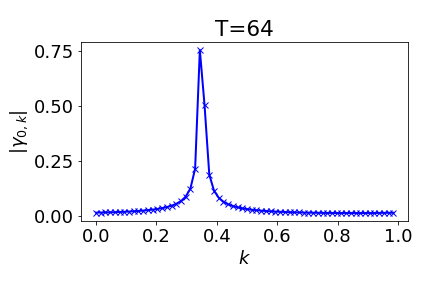
\includegraphics[width=0.4\textwidth]{qpe_gamma_T64}
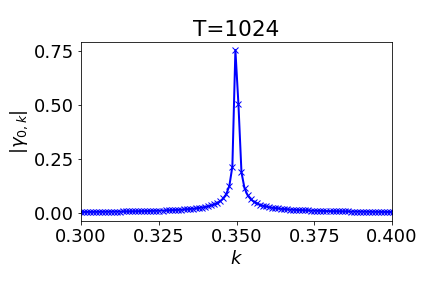
\includegraphics[width=0.4\textwidth]{qpe_gamma_T1024}
\end{center}
\caption{For $\varphi_0=0.35$, the shape of $\abs{\gamma_{0,k}}$ with $T=64$ and $T=1024$.}
\label{fig:qpe_gamma}
\end{figure}

Let $k'_0$ be the measurement outcome, which can be viewed as a random variable. The probability of obtaining some $\wt{\varphi}_{k'_0}$ that is at least $\epsilon$ distance away from $\varphi_0$ is
\begin{equation}
\begin{split}
P(\abs{\varphi_0-\wt{\varphi}_{k'_0}}_1\ge \epsilon)=&\sum_{\abs{\varphi_0-\wt{\varphi}_{k'}}_1\ge \epsilon} \abs{\gamma_{0,k'}}^2\\
\le &\sum_{\abs{\varphi_0-\wt{\varphi}_{k'}}_1\ge \epsilon}\frac{1}{4T^2 \abs{\varphi_{0} - \wt{\varphi}_{k'}}^2_1}\\
\le &\frac{2}{4T} \int_{\epsilon}^{\infty} \frac{1}{x^2}\ud x + \frac{2}{4T^2 \epsilon^2}=\frac{1}{2T\epsilon}+\frac{1}{2(T\epsilon)^2}.
\end{split}
\end{equation}
Set $t-d=\lceil\log_2 \delta^{-1}\rceil$, then $T\epsilon=2^{t-d}\ge \delta^{-1}$.
Hence for any $0<\delta<1$, the failure probability
\begin{equation}
P(\abs{\varphi_0-\wt{\varphi}_{k'_0}}_1\ge \epsilon)\le \frac{\delta+\delta^2}{2}\le \delta.
\end{equation}
In other words, in order to obtain the phase $\varphi_0$ to accuracy $\epsilon=2^{-d}$ with a success probability at least $1-\delta$, we need $d+\lceil\log_2 \delta^{-1}\rceil$ ancilla qubits to store the value of the phase.
On top of that, the simulation time needs to be $T=(\epsilon\delta)^{-1}$.

%\section{Quantum median method and high fidelity quantum phase estimation*}

\begin{rem}[Quantum median method]
One problem with QPE is that in order to obtain a success probability $1-\delta$, we must use $\log_2 \delta^{-1}$ ancilla qubits, and the maximal simulation time also needs to be increased by a factor $\delta^{-1}$. 
The increase of the maximal simulation time is particularly undesirable since it increases the circuit depth and hence the required coherence time of the quantum device.
When $\ket{\psi}$ is an exact eigenstate, this can be improved by the median method, which uses $\log \delta^{-1}$ copies of the result from QPE without using ancilla qubits or increasing the circuit depth.
When $\ket{\psi}$ is a linear combination of eigenstates, the problem of the aliasing effect becomes more difficult to handle.
One possibility is to generalize the median method into the quantum median method~\cite{NagajWocjanZhang2009}, which uses classical arithmetics to evaluate the median using a quantum circuit.
To reach success probability $1-\delta$, we still need $\log_2 \delta^{-1}$ ancilla qubits, but the maximal simulation time does not need to be increased.
\end{rem}

\vspace{2em}

\begin{exer}
Write down the quantum circuit for the overlap estimate in \cref{exam:swap_test}.
\end{exer}

\begin{exer}
For $\varphi=0.111111$, we run Kitaev's algorithm to estimate its first $4$ bits. Check that the outcome satisfies \cref{eqn:phi_kitaev_estimate}. Note that $0.0000$ and $0.1111$ are both acceptable answers.
Prove the validity of Kitaev's algorithm in general in the sense of \cref{eqn:phi_kitaev_estimate}.
\end{exer}

\begin{exer}
For a $3$ qubit system, explicitly construct the circuit for $U_{\mathrm{FT}}$ and its inverse. 
\end{exer}

\begin{exer}
For a $n$-qubit system, write down the quantum circuit for the swap operation used in QFT.
\end{exer}

\begin{exer}
Similar to the Hadamard test in \cref{exam:hadamard_qpe}, develop an algorithm to perform QPE using the circuit in \cref{fig:circ_qpe_qft} with only $d=2$, while the phase $\varphi$ can be any number in $[0,1/2)$. 
\end{exer}

